\documentclass[runningheads,a4paper]{llncs}

\usepackage[american]{babel}
\usepackage[utf8]{inputenc}

\usepackage{svg}
\usepackage{amsmath}

%extended enumerate, such as \begin{compactenum}
\usepackage{paralist}
\usepackage{color}
\usepackage{graphicx}

\usepackage{caption}
\usepackage{subfig}
\usepackage{algorithm}
\usepackage[noend]{algpseudocode}
\renewcommand{\algorithmicforall}{\textbf{for each}}
\algnewcommand\algorithmicinherit{\textbf{INHERIT:}}
\algnewcommand\INHERIT{\item[\algorithmicinherit]}
\algnewcommand\algorithmicinput{\textbf{INPUT:}}
\algnewcommand\INPUT{\item[\algorithmicinput]}
\algnewcommand\algorithmicoutput{\textbf{OUTPUT:}}
\algnewcommand\OUTPUT{\item[\algorithmicoutput]}
\makeatletter
\def\BState{\State\hskip-\ALG@thistlm}
\makeatother
\newcommand{\red}[1]{\textcolor{red}{#1}}

%put figures inside a text
%\usepackage{picins}
%use
%\piccaptioninside
%\piccaption{...}
%\parpic[r]{\includegraphics ...}
%Text...

%Sorts the citations in the brackets
%\usepackage{cite}

%for easy quotations: \enquote{text}
\usepackage{csquotes}

\usepackage[T1]{fontenc}

%enable margin kerning
\usepackage{microtype}

%better font, similar to the default springer font
\usepackage[%
rm={oldstyle=false,proportional=true},%
sf={oldstyle=false,proportional=true},%
tt={oldstyle=false,proportional=true,variable=true},%
qt=false%
]{cfr-lm}
%
%if more space is needed, exchange cfr-lm by mathptmx
%\usepackage{mathptmx}

%for demonstration purposes only
\usepackage[math]{blindtext}

\usepackage[
%pdfauthor={},
%pdfsubject={},
%pdftitle={},
%pdfkeywords={},
bookmarks=false,
breaklinks=true,
colorlinks=true,
linkcolor=black,
citecolor=black,
urlcolor=black,
%pdfstartpage=19,
pdfpagelayout=SinglePage
]{hyperref}
%enables correct jumping to figures when referencing
\usepackage[all]{hypcap}

\usepackage[capitalise,nameinlink]{cleveref}
%Nice formats for \cref
\crefname{section}{Sect.}{Sect.}
\Crefname{section}{Section}{Sections}
\crefname{figure}{Fig.}{Fig.}
\Crefname{figure}{Figure}{Figures}

\usepackage{xspace}
%\newcommand{\eg}{e.\,g.\xspace}
%\newcommand{\ie}{i.\,e.\xspace}
\newcommand{\eg}{e.\,g.,\ }
\newcommand{\ie}{i.\,e.,\ }

%introduce \powerset - hint by http://matheplanet.com/matheplanet/nuke/html/viewtopic.php?topic=136492&post_id=997377
\DeclareFontFamily{U}{MnSymbolC}{}
\DeclareSymbolFont{MnSyC}{U}{MnSymbolC}{m}{n}
\DeclareFontShape{U}{MnSymbolC}{m}{n}{
    <-6>  MnSymbolC5
   <6-7>  MnSymbolC6
   <7-8>  MnSymbolC7
   <8-9>  MnSymbolC8
   <9-10> MnSymbolC9
  <10-12> MnSymbolC10
  <12->   MnSymbolC12%
}{}
\DeclareMathSymbol{\powerset}{\mathord}{MnSyC}{180}

% correct bad hyphenation here
\hyphenation{op-tical net-works semi-conduc-tor}

\begin{document}

%Works on MiKTeX only
%hint by http://goemonx.blogspot.de/2012/01/pdflatex-ligaturen-und-copynpaste.html
%also http://tex.stackexchange.com/questions/4397/make-ligatures-in-linux-libertine-copyable-and-searchable
%This allows a copy'n'paste of the text from the paper
\input glyphtounicode.tex
\pdfgentounicode=1

\title{Onion Routing in Predictable Delay Tolerant Networks}
%If Title is too long, use \titlerunning
%\titlerunning{Short Title}

%Single insitute
\author{Adrian Antunez-Veas \and Guillermo Navarro-Arribas}
%If there are too many authors, use \authorrunning
%\authorrunning{First Author et al.}
\institute{Department of Information and Communications Engineering, \\
				Universitat Autònoma de Barcelona (UAB), 08193 Cerdanyola, Spain\\
				\email{\{aantunez, gnavarro\}@deic.uab.cat}}

%Multiple insitutes
%Currently disabled
%
\iffalse
%Multiple institutes are typeset as follows:
\author{Firstname Lastname\inst{1} \and Firstname Lastname\inst{2} }
%If there are too many authors, use \authorrunning
%\authorrunning{First Author et al.}

\institute{
Insitute 1\\
\email{...}\and
Insitute 2\\
\email{...}
}
\fi
			
\maketitle

\begin{abstract}
With the growth of Internet of Things (IoT) the data as well as the anonymity preservation has become a challenging research topic. Using Delay Tolerant Network (DTN) with onion routing an alternative secure network that hides the source identity can be achieved. We consider as predictable DTN at such networks where the behaviour is known in advance or where a repetitive action occurs over the time like in public transport networks. This project shows how the prior stage of path choosing in the onion routing can be achieved using the information provided by predictable networks while the security of our proposed method is analysed.
\end{abstract}

\keywords{Onion Routing, Delay-tolerant Network, Anonymous networking, Privacy, Security}

\section{Introduction}\label{sec:intro}

\red{Delay Tolerant Networks (DTNs) are a class of networks aimed to provide end-to-end communication into environments lacking continuous connectivity or with long delays. DTNs can also be used as a communication alternative when the internet internet network can not be trusted, e.g: unknown Wi-Fi hotspots.}

\red{DTNs use the store-carry-and-forward principle, i.e: the node stores the message (bundle) received , carrying it if is needed and forwarding it when a connection opportunity occurs.}

\red{Due to the nature of the DTNs the routing decision has been challenging since the beginning.}

\red{The main problem w this kind of networks is mainly the routing and the security of the data exchanged. On the one hand due to the nature of the nodes of the DTN could be under continuous movement making the routing of the data a difficult task. On the other hand \red{\ldots}}

\red{Onion routing is used to protect the communications online allowing to hide the origin or the source of the information as well as the data itself to the rest of the nodes that forwards the information.}

\red{DTN Oracle: Information of the network as contact information (time of the contact and duration) and the public key of every single node of the network, in order to be able to do the Onion Routing.} 

\section{Related work}\label{sec:rwork}

\red{Related work goes here}.

\section{Proposal}\label{sec:proposal}

\red{Proposal goes here}.

\section{Security analysis}\label{sec:sanalysis}

%\red{Aim of this section: •.}

In this section, we evaluate our proposed scheme from the aspect of security. First, we define the threat model, defining important considerations regarding the scenario under study. After, we define different kinds of adversaries explaining what they can do and what we do to preserve the sender anonymity as well as the privacy of exchanged information.

\subsection{Threat model}

Alice (\textit{A}) wants to communicate to Bob (\textit{B}) without revealing information about her. Using onion routing we intend to improve A's anonymity as well as data privacy against adversaries that can be passive,i.e: eavesdropping messages or take an active paper in this scenario, i.e: make modifications or attack to other nodes of the network. In general, security threats can be divided into passive and active threats. We consider that nodes in our scenario use strong cryptographic algorithms with enough key lengths to prevent practical cryptanalysis attacks to discover the source, the destination or the contents of a message. 

\subsection{Passive adversaries}

Passive attacks are those that perform guessing simply observing user traffic patterns from "passive" nodes. 

As is explained in \cite{latency-leak} if the attacker is the destination of the message, he can learn something from the delay between messages.  This kind of attacks does not work when sending start time, known as \textit{t} parameter in our path choosing method, is not highly predictable \cite{enpassant}.

Another attacker model is a set of compromised nodes that works together to retrieve information leading to break the users privacy. We have two different situations to deal with: the multiple decryption and the sending node periodicity. First, the attacker will be able to decrypt more layers, or messages if one of the nodes is the destination, because they have their corresponding private keys. Second, there are scenarios where a node or a set of them rarely transmit information to others, discarding this nodes from the probable sending set, a globally passive adversary can correctly guess the source of a message. To overcome such attacks the \textit{n} value can be increased, i.e: the number of nodes that has a single path to send the message. As much nodes, much layers a message will have. There is a trade-off between efficiency and security deciding \textit{n} value. To solve the guessing issue the creation of dummy packets when ingress throughput drops below a certain threshold \cite{arden} may help to prevent such attacks.

Is important to note that an attacker can combine previously explained attacks to increase their chance of guessing.

To decrease the probability of guess the path, different paths are retrieved using our path choosing method and one of them is chosen randomly.

\subsection{Active adversaries}

Active adversaries are those that performs actions against other nodes or modifies information that cross through them. As is the case of passive nodes, an attacker controlling a single node will be unable to extract the source of a message because of the use of multiple layers of encryption \cite{arden}. There are several possible attacks to do against onion routing by malign node in the network \cite{congestion-attack}, \cite{location-attack}, \cite{latency-leak}.

An attacker who has a control of a node of the network can attacking non-observed nodes to shut them down. Prohibiting the communication between the source and the destination if that node was implied in involved in the chosen path. This kind of attacks are called Denial of Service DoS attacks and can be addressed improving the robustness of the nodes as well as with reputation systems as in discussed in conclusions and future work section \ref{sec:conclusions}.

Message modifications by attackers are easily detected using cryptographic hash methods. Other attacks like masquerading (nodes pretending to be different nodes) are solved as layers of encryption check the node identity. The key management process is safely done in a prior stage.

\section{Evaluation}\label{sec:evaluation}
%\red{Aim of this section: •.}

%\red{Aim of this section: Brief introduction of what are we going to talk about in this section.}

% ns-3: https://www.nsnam.org/
In this section we conduct simulation based on realistic scenario trace file to verify the feasibility of our proposal. We decided to recreate the small public transport network of the UAB campus using the Network Simulator 3 (NS-3). NS-3 is a well-known discrete-event simulator targeted primarily for the research usage~\cite{ns-3-webpage}. We explain as well how the mobility model was obtained as well as what parameters were used during the simulation. Finally we will test our proposed method in the simulation to evaluate how it performs.

\subsection{Scenario: Campus buses}

%\red{Aim of this section: Explain a bit how the campus scenario works and how can be this useful in practice.}

In order to test our proposal we considered a very small public transportation network that works inside the Autonomous University of Barcelona (UAB) composed by 5 buses that makes different routes around the UAB campus. Is important to note that every single bus makes the same route daily. By this way, this example can be seen as a good example of deterministic networks.

Each bus has a DTN node that allows to achieve secret communications as well as source anonymity using onion routing protocol. There are several applications that can take profit of such networks like anonymous reporting systems.

\subsection{Mobility Model}

%\red{Aim of this section: explain how we get this scenario: open street maps -> sumo -> ns-3... }

We obtained the mobility model going through different stages. First, we exported the UAB Campus map from OpenStreetMaps into SUMO software~\cite{sumo}, filtering some unnecessary items like buildings and railways with the Java OpenStreetMap editor tool~\cite{josm}.

% bus-schedule: http://www.uab.cat/doc/horaris_busUAB_2015
Once the campus roads were imported in SUMO, we recreated the bus movements of each bus taking into consideration the official bus schedule of the UAB public transportation network \cite{bus-schedule}. In addition, we tuned some bus characteristics like acceleration and deceleration parameters in order to get coherent travel times.

%sumo-to-ns-2: http://www.ijarcsse.com/docs/papers/Volume_4/4_April2014/V4I4-0416.pdf
Finally, we exported the model to a NS-2 mobility trace as is explained in \cite{sumo-to-ns-2}. The NS-2 mobility trace can be used in NS-3. We used the simulator to obtain important contact related data of the campus network, i.e: information about the duration of the contacts as well as the instant of time when they occurred.

\subsection{Simulation setup}

%\red{Aim of this section: Explain and define the values used in the simulation itself as well as how we know that there is a neighbour able to contact with.}

% ns-3-dtn: https://www.nsnam.org/wiki/Current_Development
The DTN modules are under current development in NS-3 \cite{ns-3-dtn}. For this reason we decided to implement a neighbour discovery in the application layer. This application broadcasts beacons messages periodically looking for new contact opportunities. The interval time is the time to wait between beacons while the expiration time is the time a neighbour is considered valid, these parameters can be set up manually.

\begin{table}[h]
\centering
\begin{tabular}{l|l}
Parameter & Value \\
\hline
Number of nodes & 5 \\
Wi-Fi range & 100 meters \\
Interval time & 1 second \\
Expiration time & 2 seconds \\
Simulation time & 15 hours \\
DSS Rate & 1 Mbps \\
IEEE 802.11 specification & 802.11b
\end{tabular}
\caption{Simulation setup.}
\label{table:simulation-parameters}
\end{table}

As can be seen in table~\ref{table:simulation-parameters}, we also tuned different wireless parameters to be suitable with resource-constrained computers like those that could be used in each bus.

\subsection{Simulation results}

%\red{Aim of this section: Explain the results of this simulation. What we get explaining why.}

In figure~\ref{fig:contact-duration-group} we have an overall view of the network activity. There is a group that have really short contact times, these contacts can be suitable for those applications that does not require a huge amount of data to send. There is another group that has long contact times (nearly 7 minutes), these group is able to perform complex communications sending higher amount of data. The average contact time is near 1 minute indeed is suitable for several applications like anonymous reporting systems. A summary of contacts related information during the simulation is shown in table~\ref{table:contact-information}. With this simple network characterization we show that our evaluation model can be used for several applications. 

\begin{table}[h]
\centering
\begin{tabular}{l|l}
Metric & Value \\
\hline
Number of contacts & 1161 \\
Average contact time  & 72.72 seconds \\
Maximum contact time &  412 seconds\\
Minimum contact time &  1 second
\end{tabular}
\caption{Contact information.}
\label{table:contact-information}
\end{table}

\begin{figure}[hbt]
  \centering
  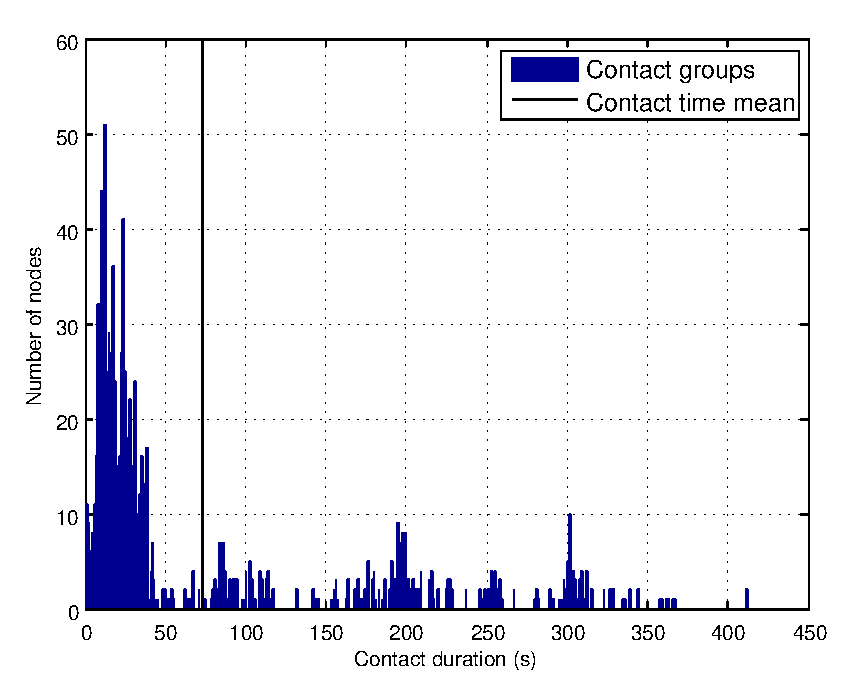
\includegraphics[scale=0.70]{imgs/statistics/contats-duration}
  \caption{Number of contacts with the same duration.}
  \label{fig:contact-duration-group}
\end{figure}


\red{Create a ratio between time and probability to guess the source. Normalize the value between 0 and 1. Do a 3-D graphic modifying k and n. Normalize like \url{https://docs.tibco.com/pub/spotfire/5.5.0-march-2013/UsersGuide/norm/norm_scale_between_0_and_1.htm}}

\section{Conclusions}\label{sec:conclusions}

\red{Conclusions goes here}.

\subsubsection*{Acknowledgements}

\red{Acknowledgements go here}.

%%%%%%%%%%%%%%%%%%%%%%%%%%%%%%%%%%%%%%%%%%%%%%%%%%

\bibliography{paper}

All links were last followed on \today.

\bibliographystyle{ieeetr}

\end{document}
